\chapter[Realizacja sonaru ultradźwiękowego]{Realizacja sonaru ultradźwiękowego}

\label{chapter:realizacja}
Obwód drukowany został zamówiony w zagranicznej firmie JLCPCB \cite{jlcpcb}. Niektóre opcje transportowe oferują korzystne czasy realizacji, 
wynoszącę nawet do jednego tygodnia, będąc tym samym dużą konkurencją wobec lokalnych producentów. Kolejnym czynnikiem 
wpływającym na decyzję wyboru jest cena. Dzięki optymalizacji procesów produkcyjnych podstawową płytkę dwuwarstwową można zamówić już nawet za 2\$, 
podczas gdy lokalnie cena jest co najmniej dziesięciokrotnie wyższa.
Przekłada się to na popularność głównie chińskich dostawców wśród zarówno amatorów elektroniki, jak i profesjonalistów.
JLCPCB posiada również w swojej ofercie montaż maszynowy elementów elektronicznych. Wymaga to dostarczenia odpowiednich plików produkcyjnych i listy materiałowej. 
Koszt montażu i komponentów jest doliczany do rachunku. Pozwala to zaoszczędzić bardzo dużo czasu podczas całego procesu wdrażania urządzenia. 

W celu obniżenia kosztów produkcyjnych, wszystkie płytki składowe projektu zostały zawarte w jednym arkuszu tak jak widać na rysunku \ref{fig:pcb}. Producent traktuje to jako jedno zlecenie, oraz nie ma potrzeby 
wielokrotnego konfigurowania maszyny pod montaż elementów. Łączenia miedzy modułami zostały zaprojektowane tak, aby nie stwarzały ryzyka oderwania podczas produkcji, 
ale jednocześnie by można było je celowo łatwo rozdzielić ręcznie. 

\begin{figure}[ht!]
    \centering
    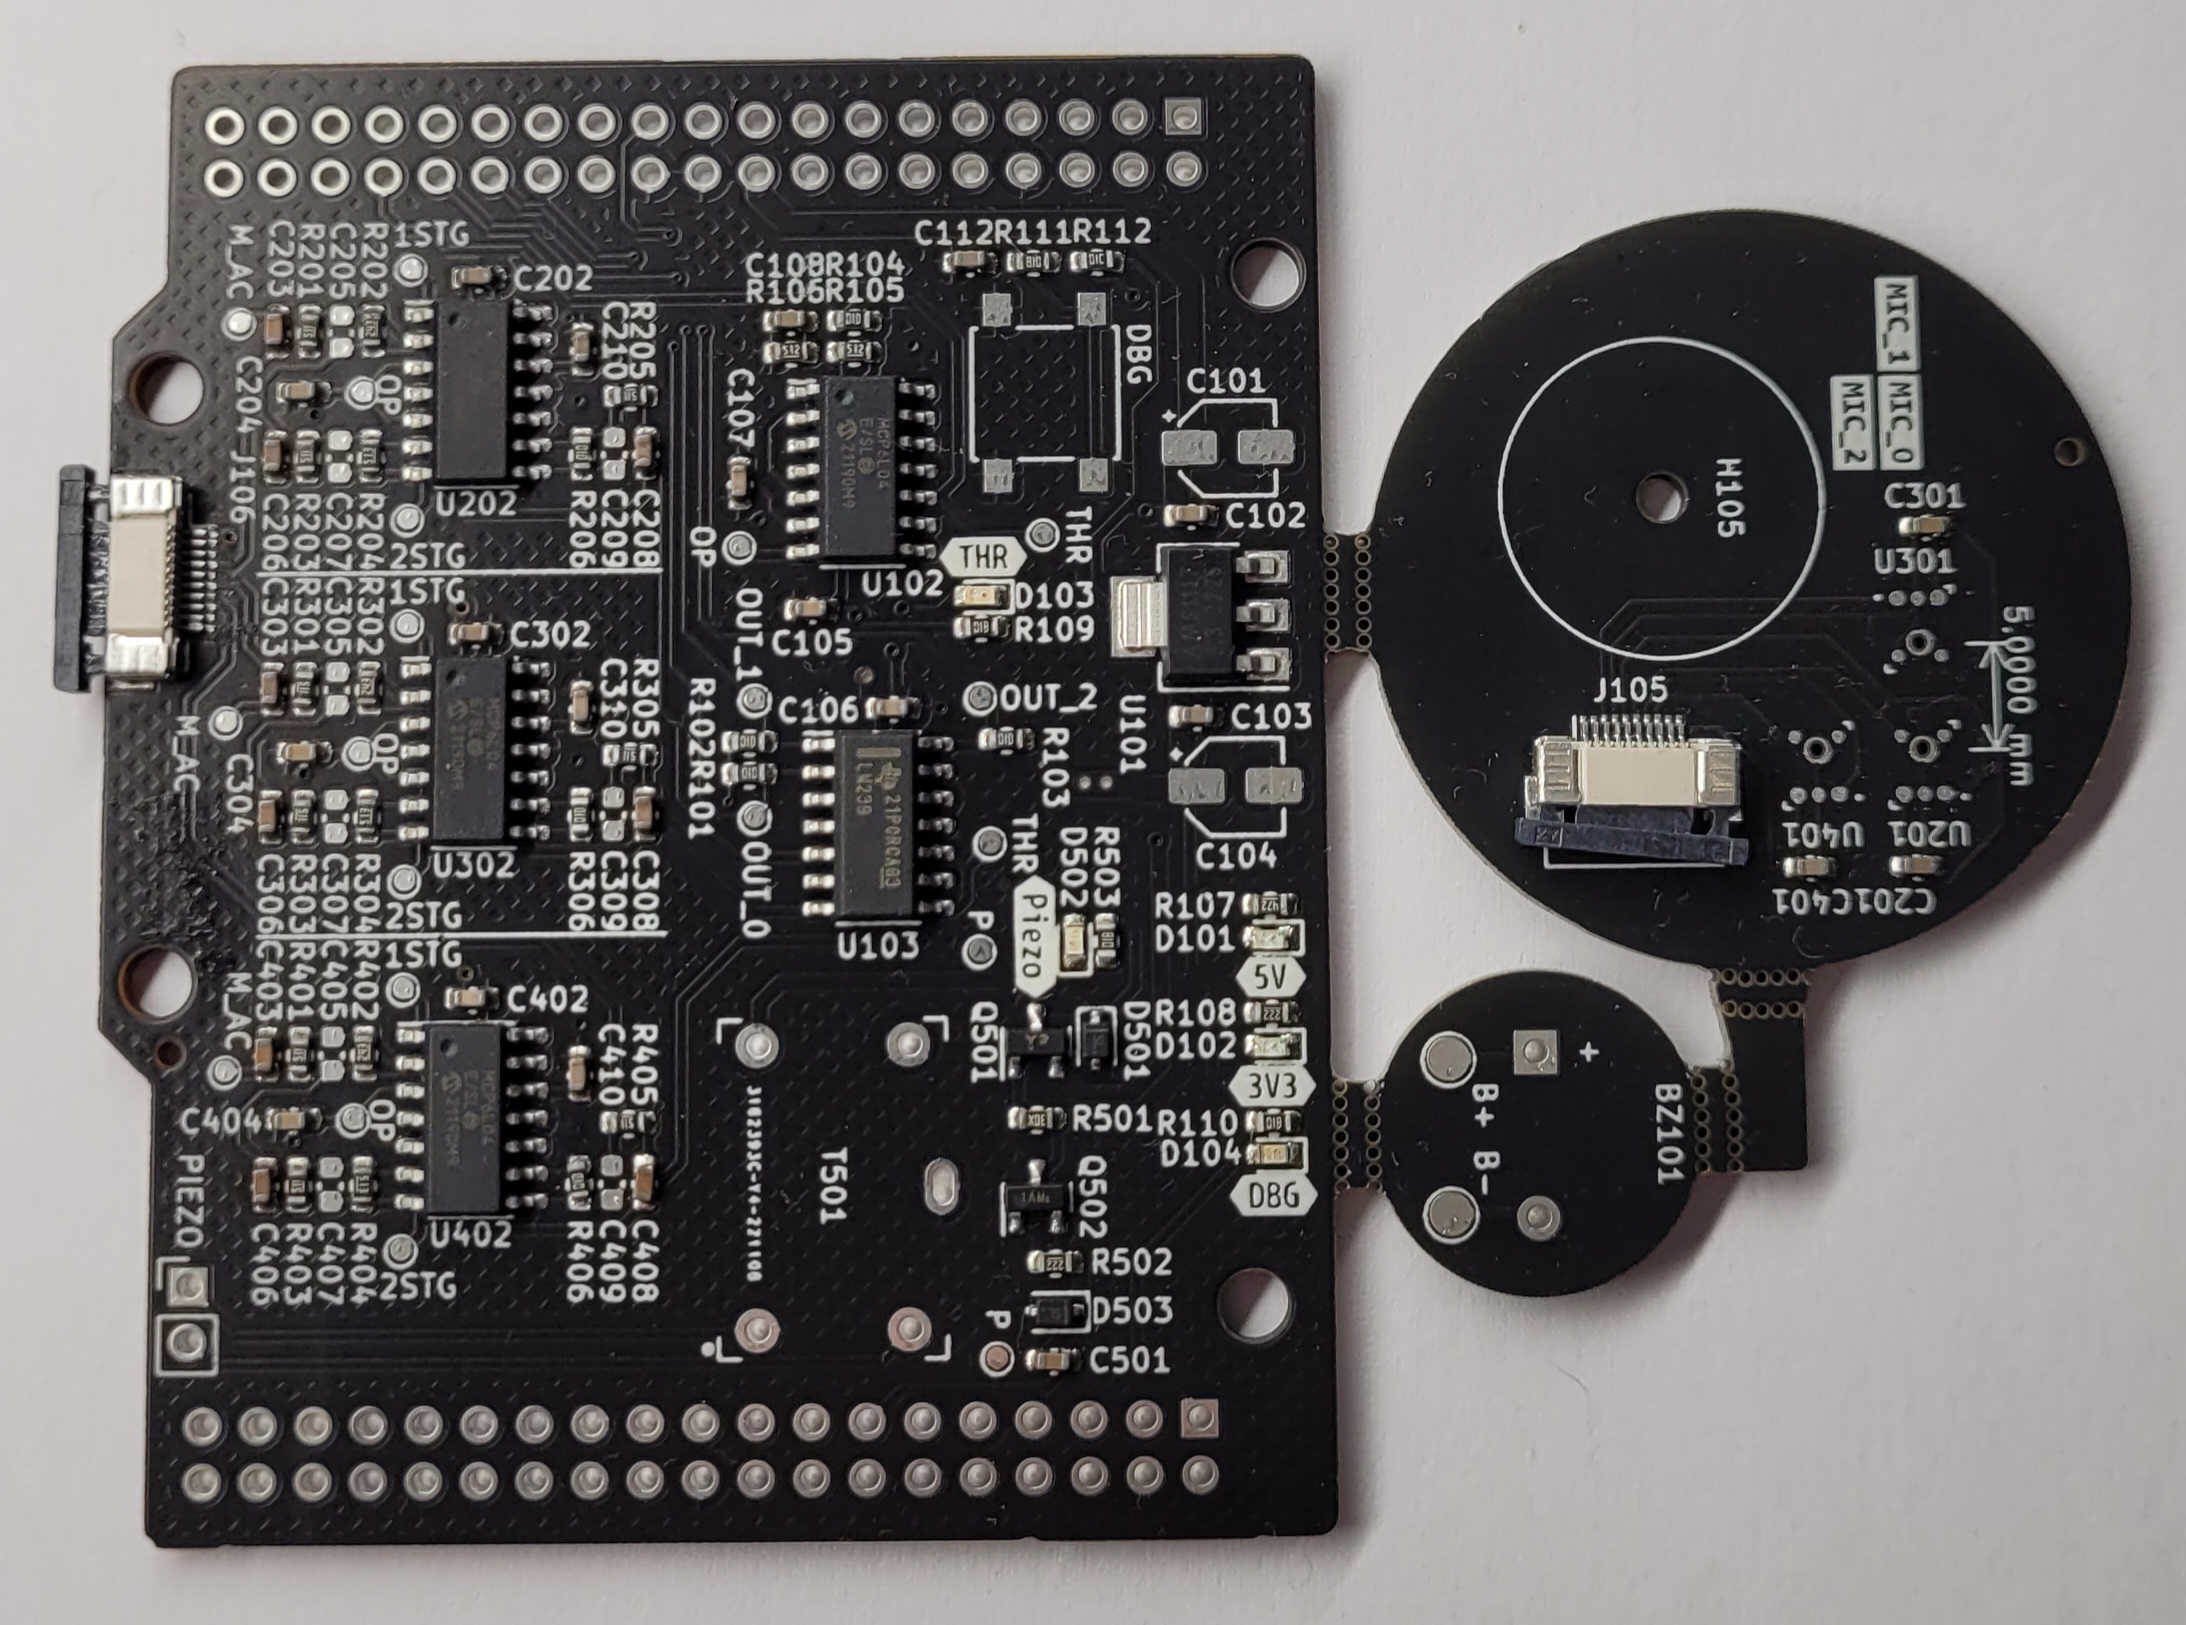
\includegraphics[width=0.55\textwidth]{jlc.jpg}
    \caption{PCB}
    \label{fig:pcb}
\end{figure}

\clearpage
Moduł z przetwornikami jest okrągłą płytką widoczną na rysunku \ref{fig:nadajnikodbiornik}, na której mieści się przetwornik umieszczony w dużym otworze, 
mikrofony których układ sugerują trzy małe otwory, pełnią one funkcję kanału ciśnieniowego, to dzięki nim dźwięk dostaje się do mikrofonów będących po drugiej stronie płytki.
Z głównym modułem łączy się przez taśmę FPC o rastrze \unit[0,5]{mm}. Celem tworzenia osobnego modułu dla przetworników dźwięku jest konieczność umiejscowienia tych elementów 
na zewnątrz obudowy oraz skierowania ich w kierunku pracy urządzenia.

\begin{figure}[ht!]
    \centering
    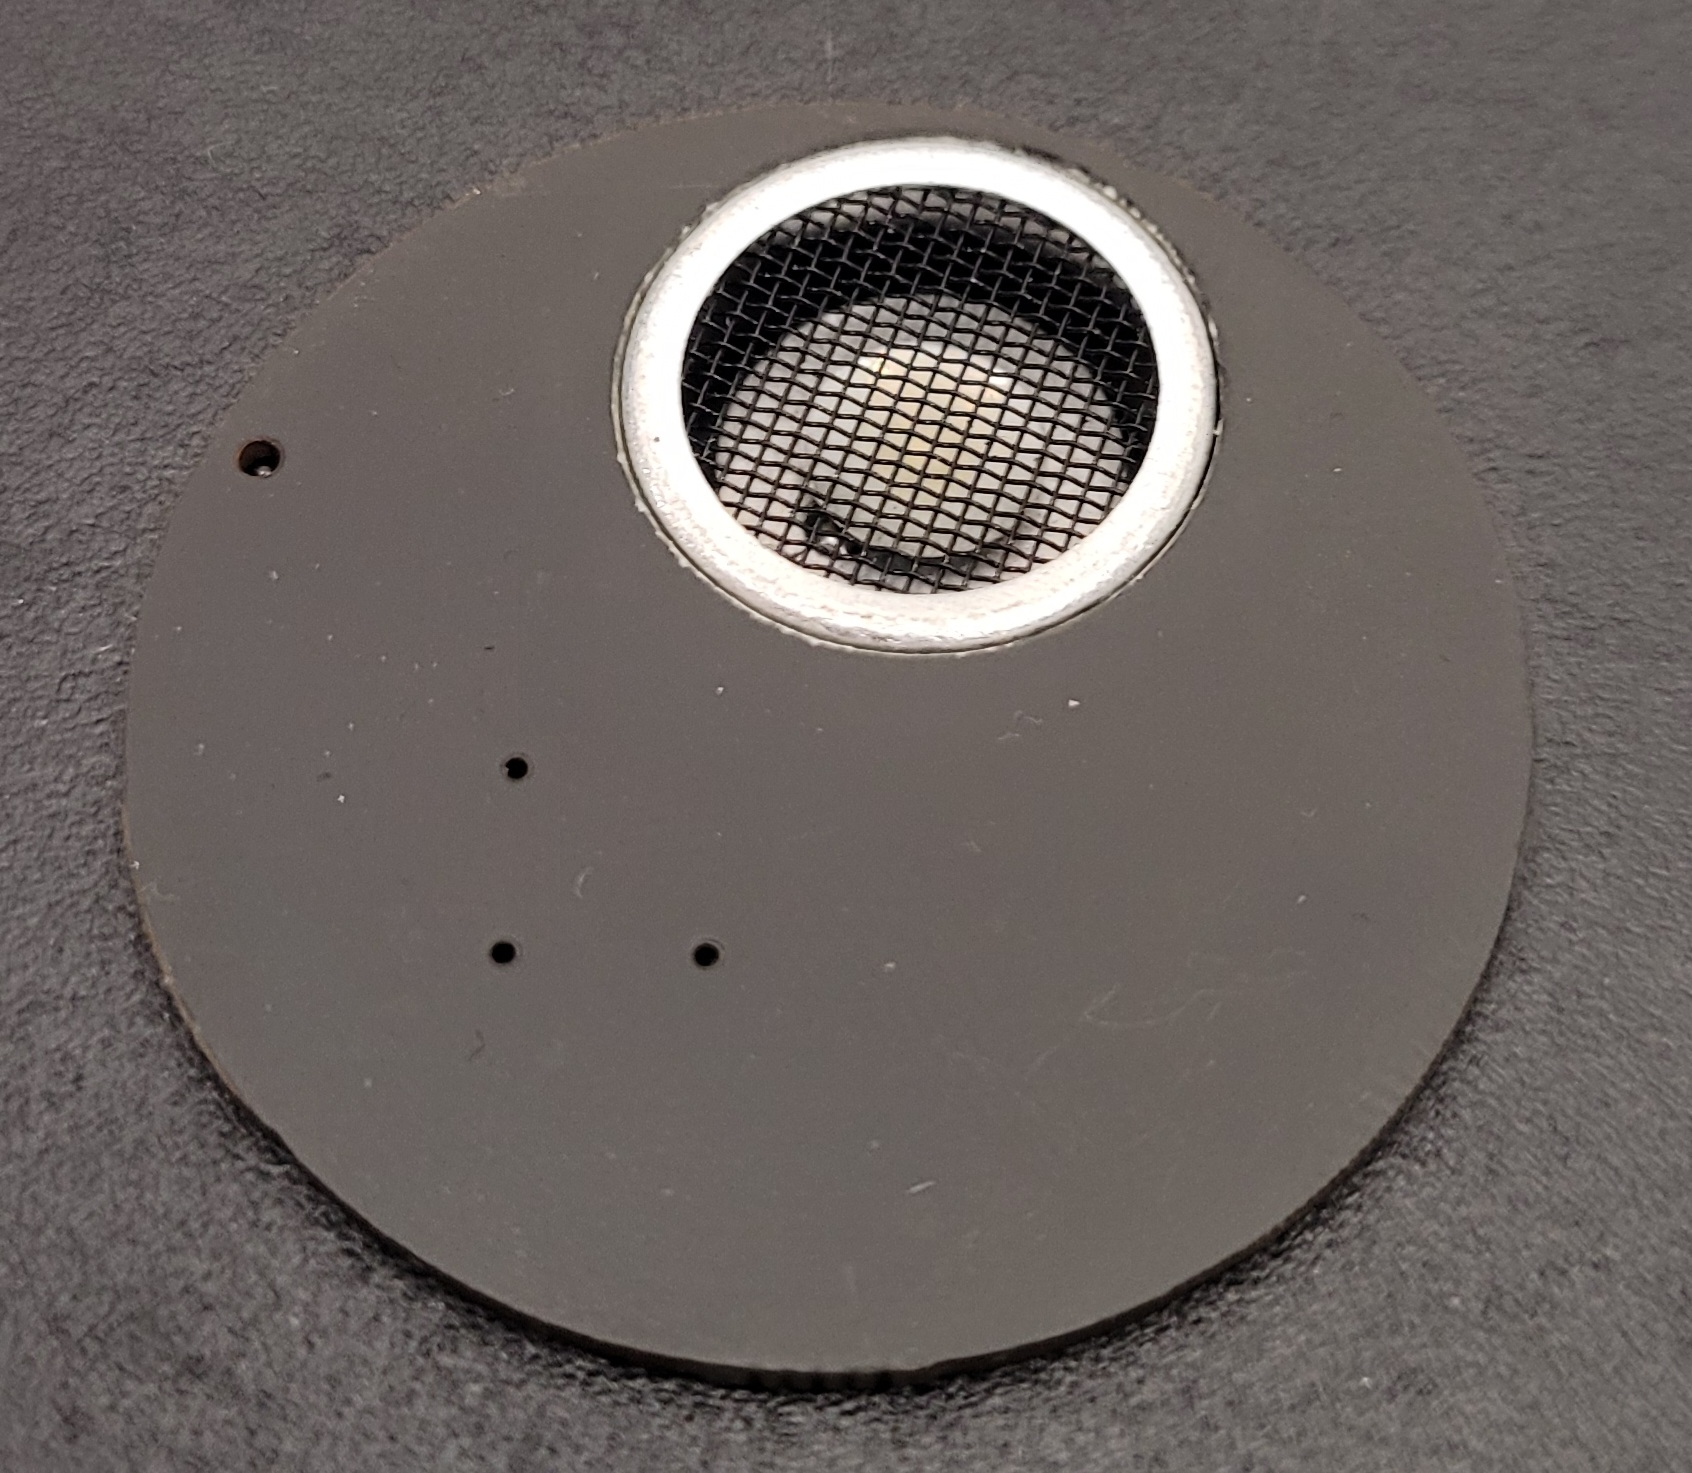
\includegraphics[width=0.4\textwidth]{nadajnikodbiornik.jpg}
    \caption{Moduł nadawczo-odbiorczy}
    \label{fig:nadajnikodbiornik}
\end{figure}

Główny moduł został zaprojektowany na wzór popularnych w prototypowaniu nakładek na płytki deweloperskie. 
Tak jak widać na rysunku \ref{fig:shieldnucleo} obwód drukowany jest nałożony bezpośrednio na taką płytkę, bez konieczności użycia przewodów.  
Moduł łączy się z Nucleo poprzez listwy kołkowe na które wyprowadzone zostały prawie wszystkie piny mikrokontrolera STM32L476 oraz dodatkowo napięcia zasilające całą płytkę.
Umieszczono tutaj cały układ wzmacniacza nadajnika oraz filtry, wzmacniacze i komparatory należące do bloku odbiorczego. 
Na krawędzi umieszczone są złącza służące do podłączenia nadajnika i odbiorników urządzenia.

\begin{figure}[ht!]
    \centering
    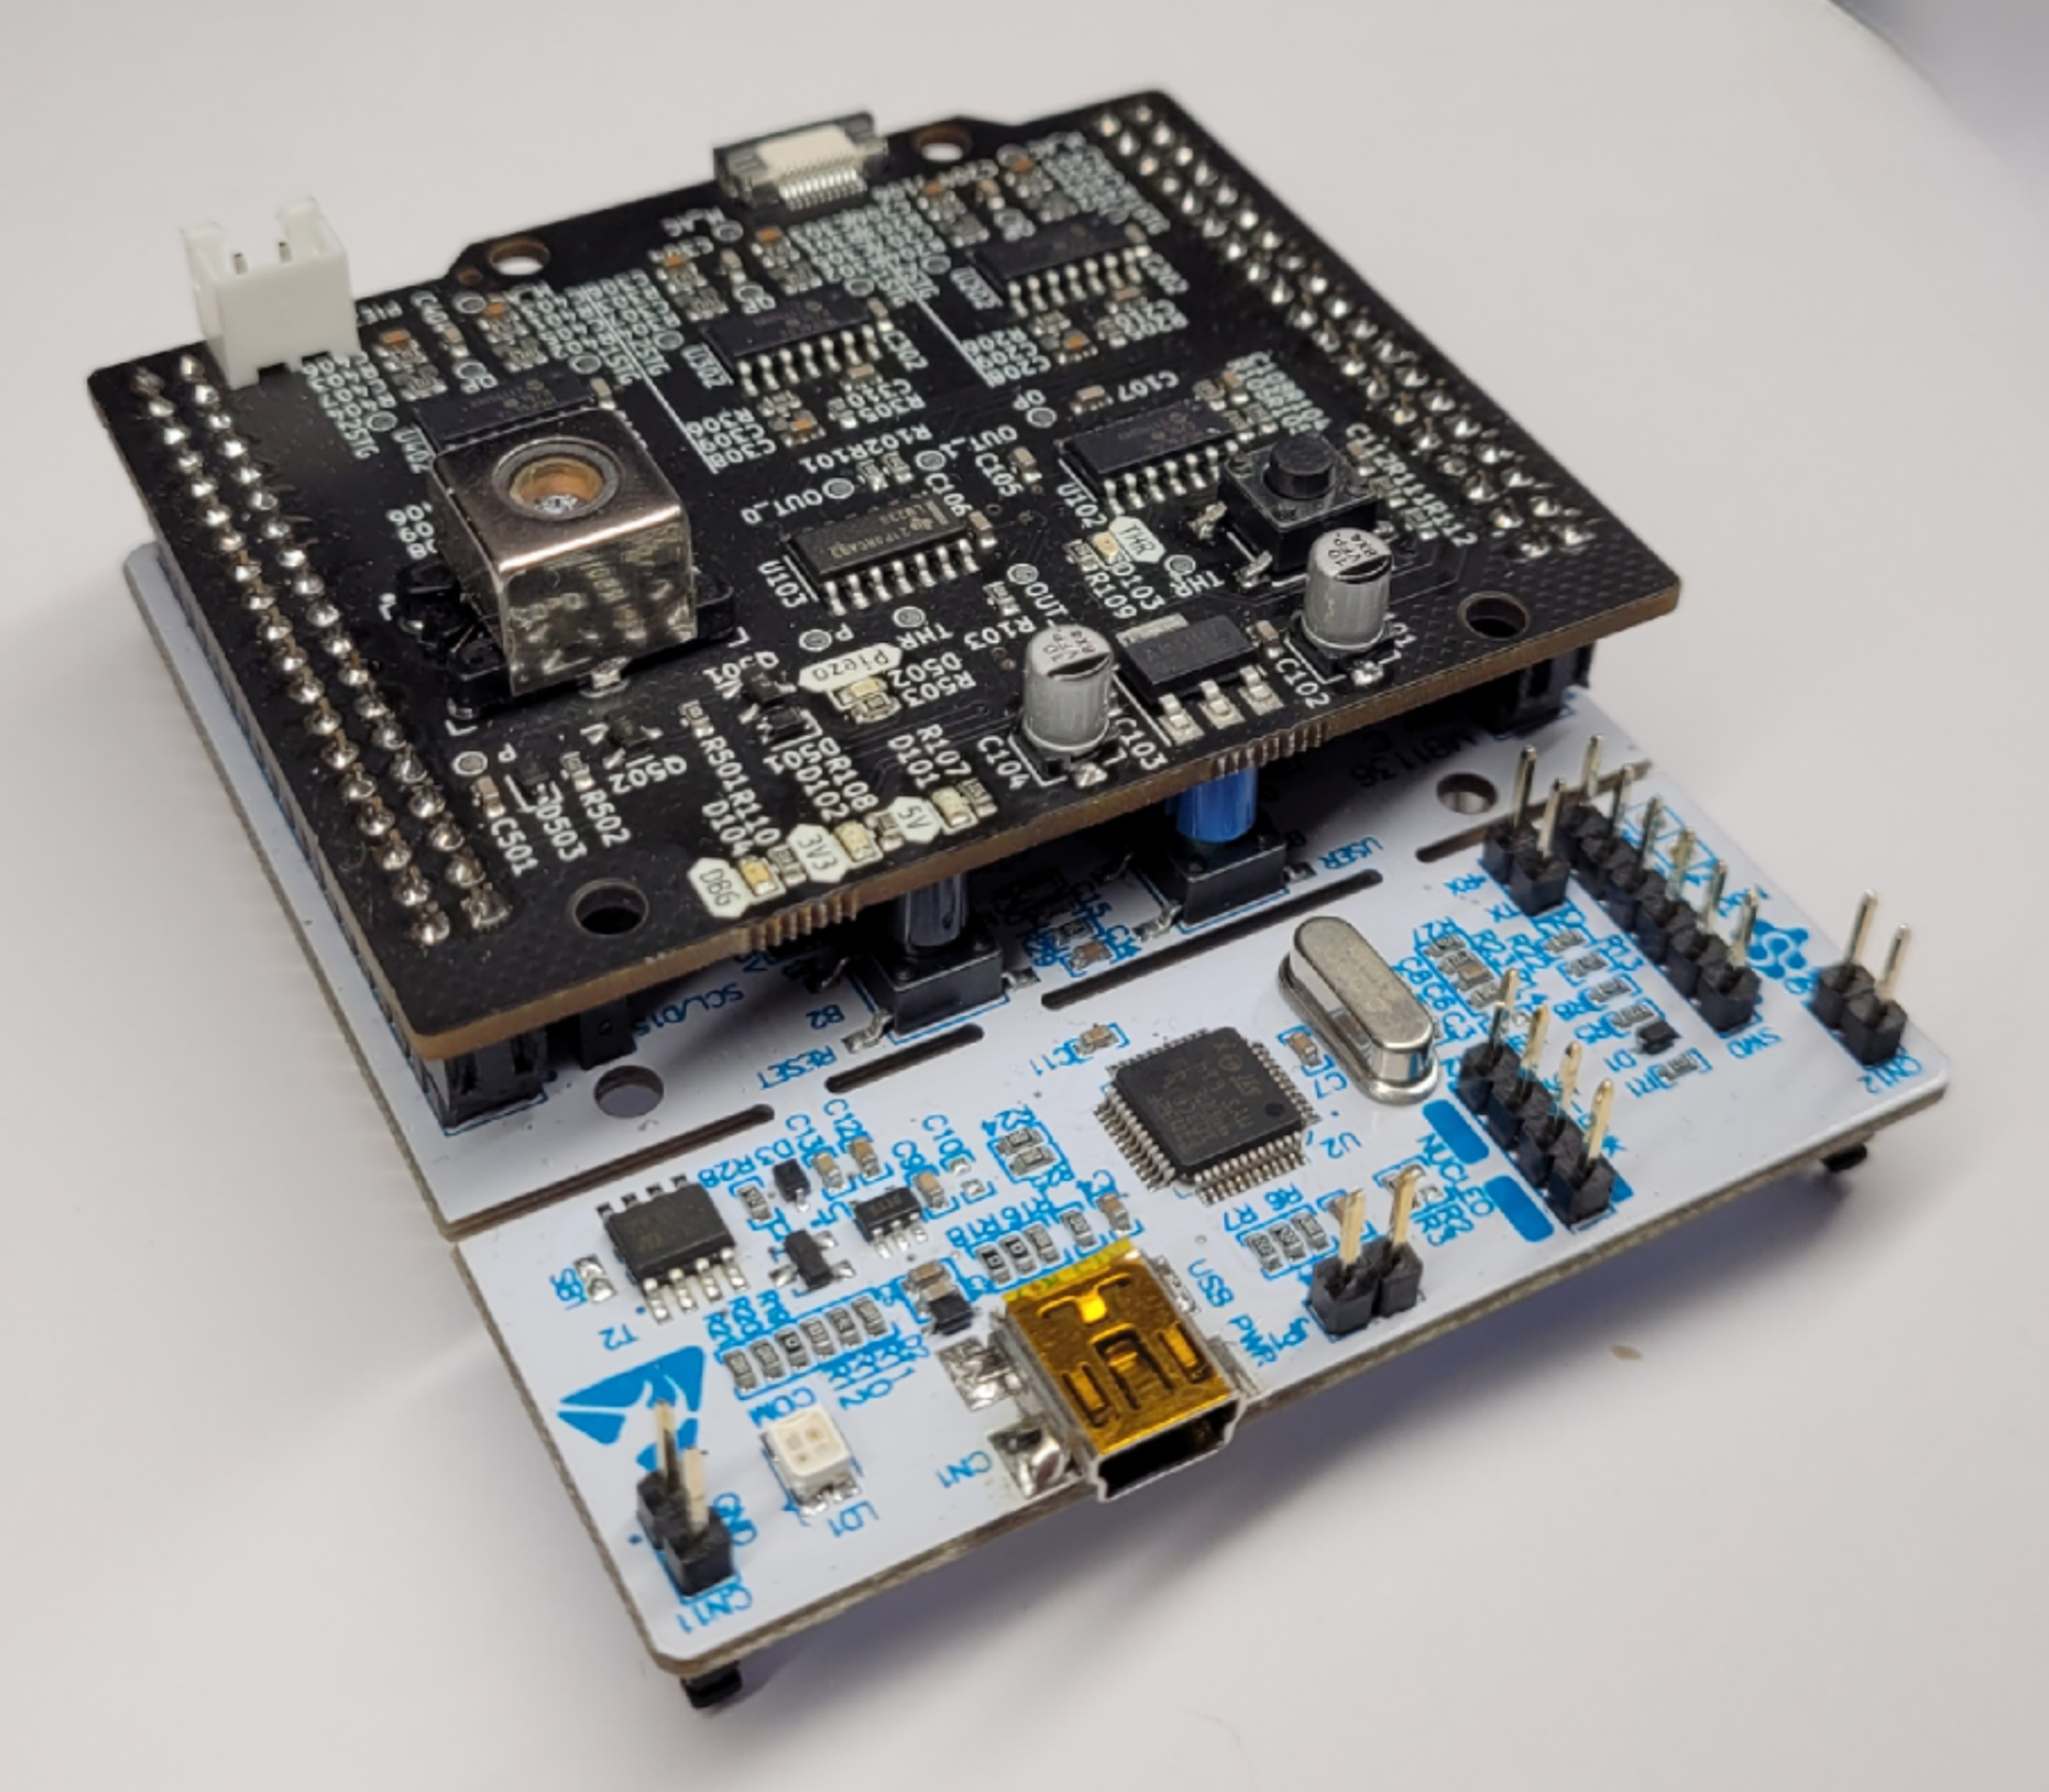
\includegraphics[width=0.5\textwidth]{shieldnanucleo.jpg}
    \caption{Nakładka na Nucleo}
    \label{fig:shieldnucleo}
\end{figure}

\clearpage
Całe urządzenie zostało umieszczone w plastikowej obudowie marki KRADEX \cite{kradex}. Dostępne są one w wielu wariantach wymiarów, 
kształtów oraz materiałów. Ułatwiło to znalezienie modelu, który będzie najbardziej odpowiedni do tego zadania. Materiał obudowy został wybrany ze względu na łatwość obróbki, 
a także na konieczność wywiercenia dodatkowych otworów na moduł nadawczo-odbiorczy bądź na port USB widocznych na rysunku \ref{fig:done_open}.
Do montażu płytki deweloperskiej wykorzystane zostały przeznaczone do tego otwory montażowe na laminacie. Za pomocą dystansów płytka została przykręcona do obudowy, 
a moduł nadawczo-odbiorczy został zamocowany do górnej jej części za pomocą kleju. 
Inne sposoby mocowania tego modułu takie jak śruby, mogłyby zakłócić pomiar poprzez odbicia od ich powierzchni w pobliżu mikrofonów. 

\begin{figure}[ht!]
    \centering
    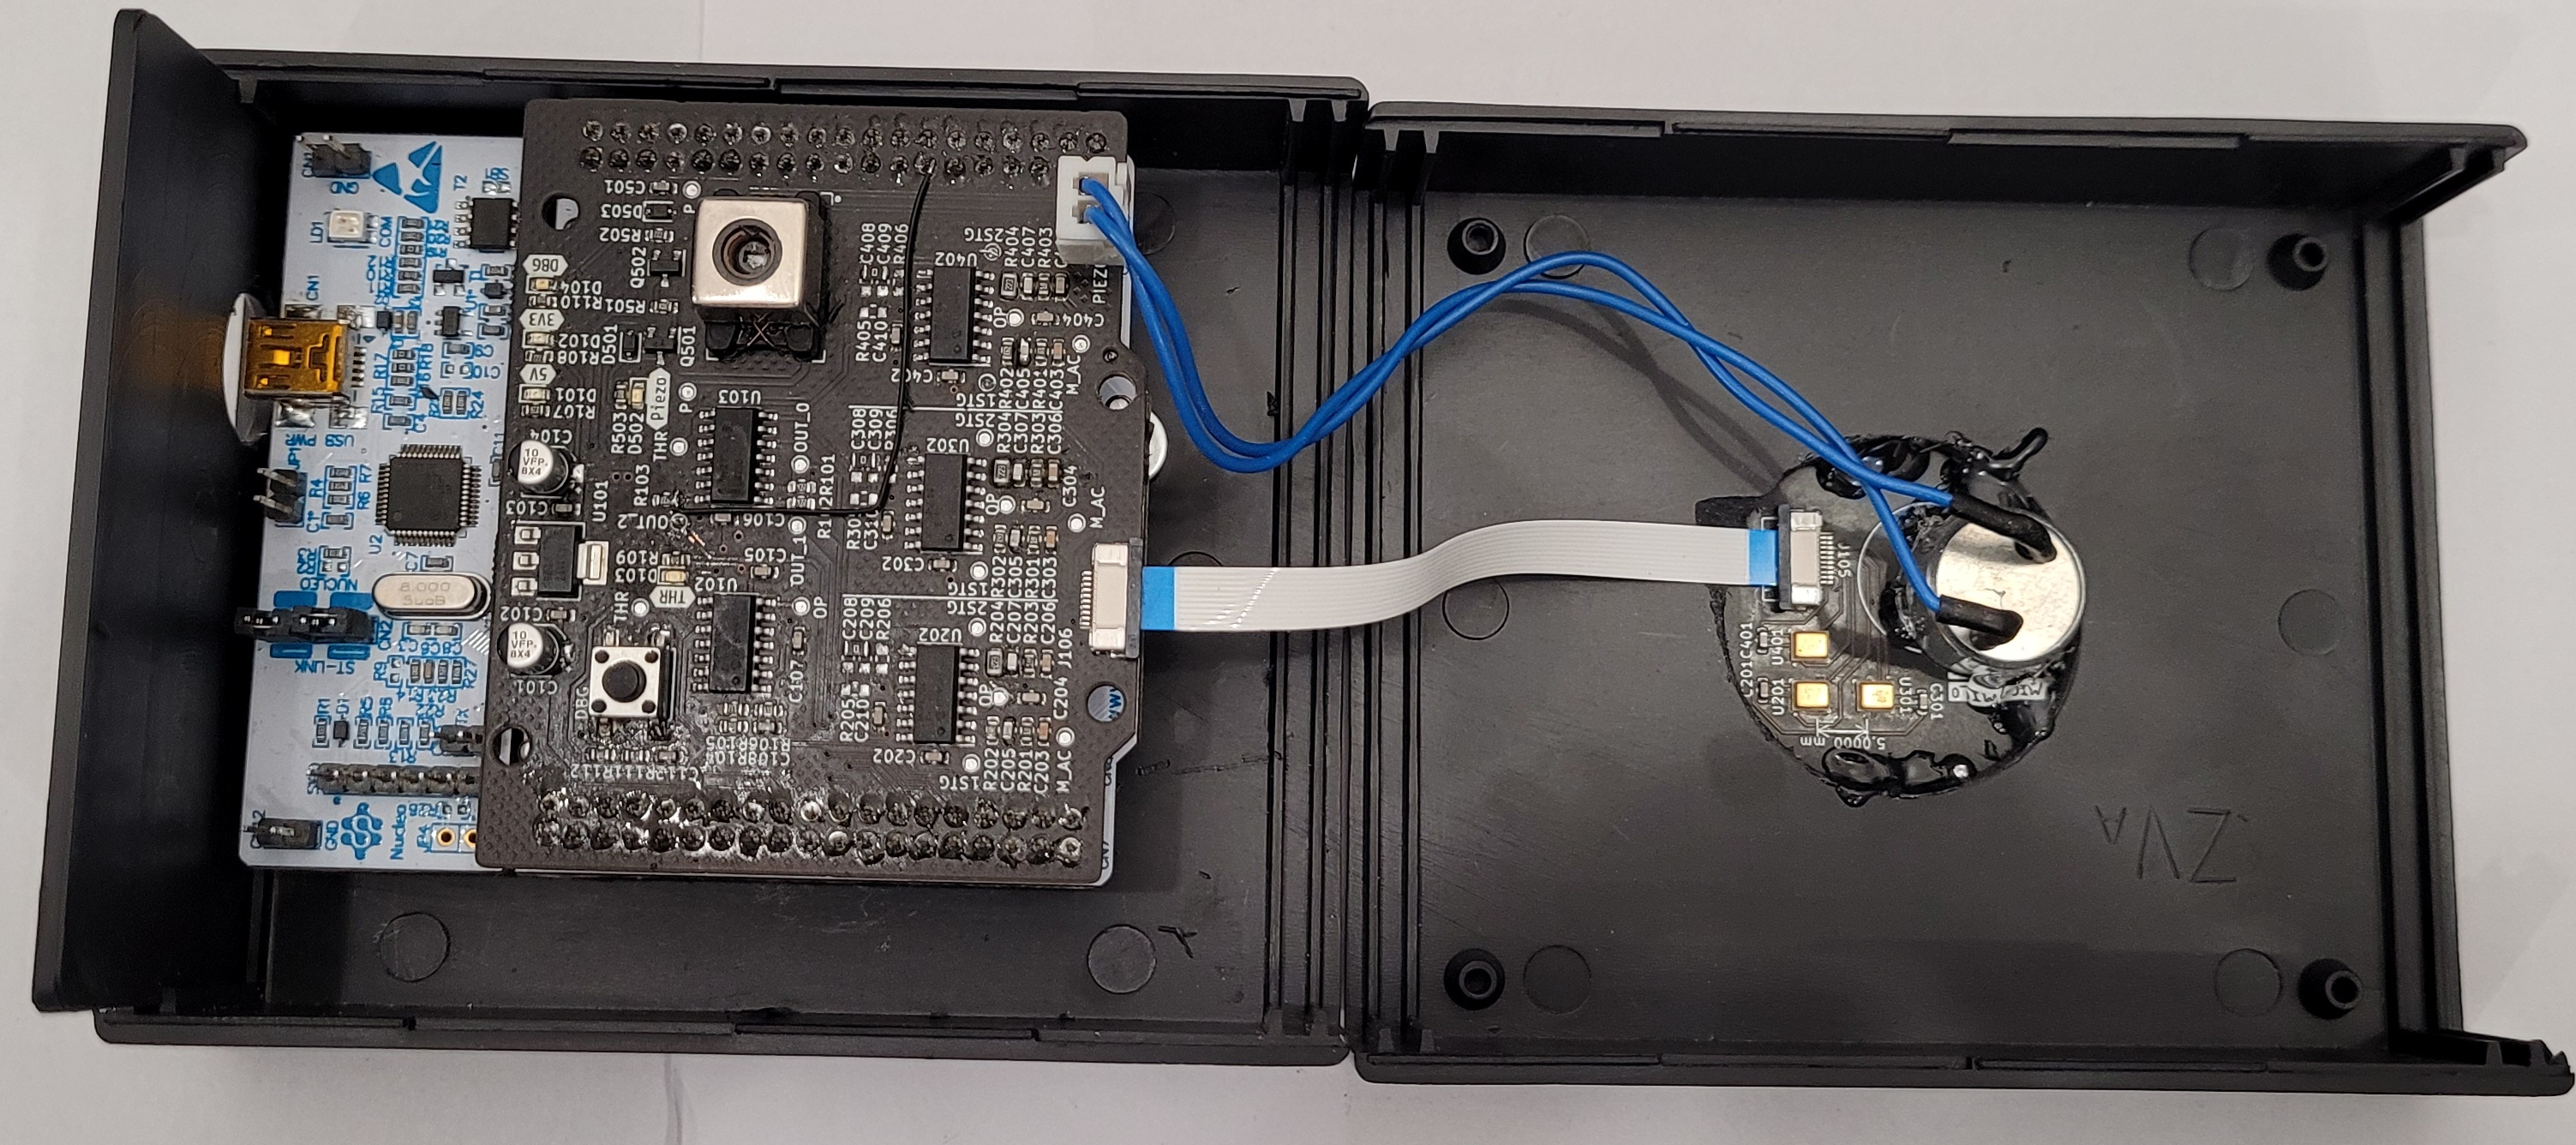
\includegraphics[width=0.8\textwidth]{doneotwarte.jpg}
    \caption{Skończony projekt w otwartej obudowie}
    \label{fig:done_open}
\end{figure}

W sposób ukazany na rysunku \ref{fig:done} prezentuje się gotowe urządzenie. Jak widać, czoło urządzenia jest możliwie płaskie by jak najmniej zakłócać pomiar.
Sonar względem użytkownika udostępnia tylko złącze mini USB w celu komunikacji i zasilania urządzenia. Cała interakcja odbywa się za pomocą oprogramowania.

\begin{figure}[ht!]
    \centering
    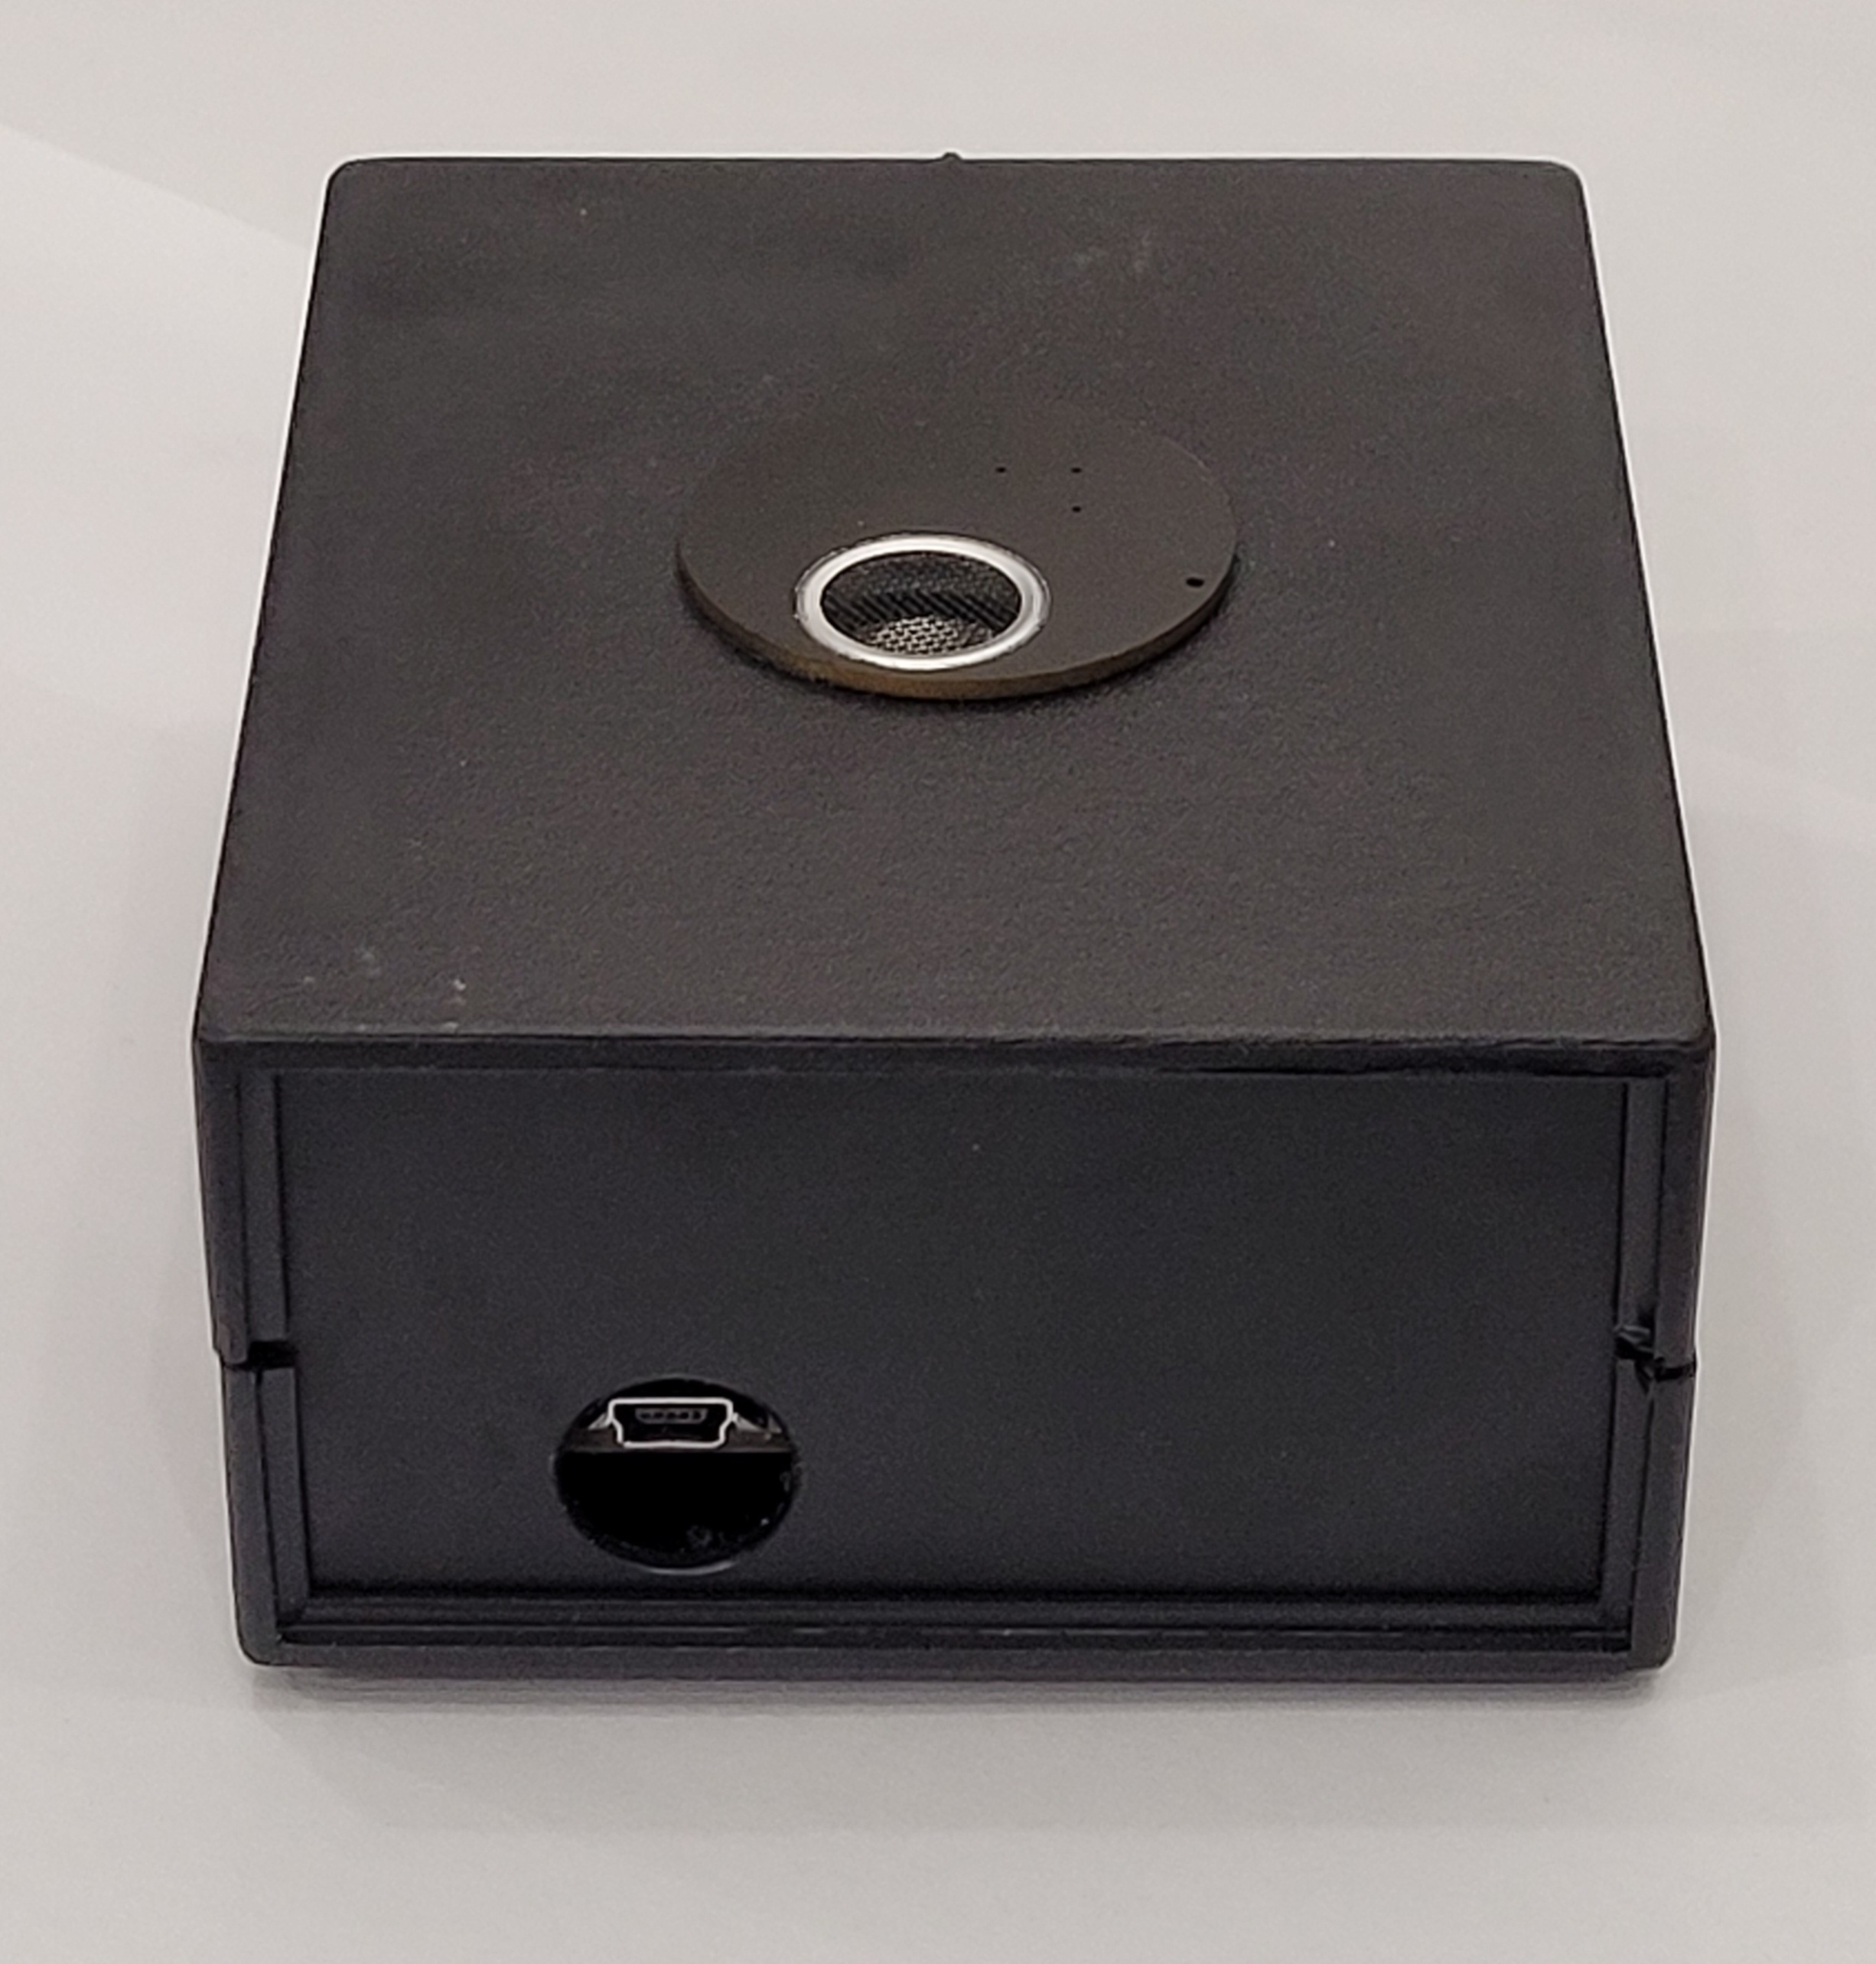
\includegraphics[width=0.4\textwidth]{donezamkniete.jpg}
    \caption{Skończony projekt}
    \label{fig:done}
\end{figure}
\clearpage
Na zrzucie ekranu widocznym na rysunku \ref{fig:comm} przedstawiona została przykładowa komunikacja z urządzeniem. 
Pierwsza odebrana wiadomość to komenda "4" z parametrem "2800". Oznacza to, 
że próg wykrywania impulsu został zmieniony na wartość 2800 jednostek, o czym program poinformował w wiadomości będącej odpowiedzią na tę komendę.
Następnym przechwyconym ciągiem znaków jest "X 0 0", co przekłada się na komendę numer 0, która nie przyjmuje żadnych parametrów, dlatego też w jego polu również przekazane zostało zero.
Komenda ta oznacza polecenie uruchomienia sekwencji pomiarowej sonaru. W odpowiedzi na pomiar powinien być zwrócony wynik pomiaru również w formie tekstowej.
\begin{figure}[ht!]
    \centering
    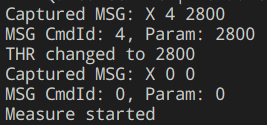
\includegraphics[width=\textwidth]{comm.png}
    \caption{Widok terminala podczas komunikacji z urządzeniem }
    \label{fig:comm}
\end{figure}
